\section{Results}
\label{sec-results}
\input graphsize_table

\begin{figure*}[t]
       \begin{center}
                       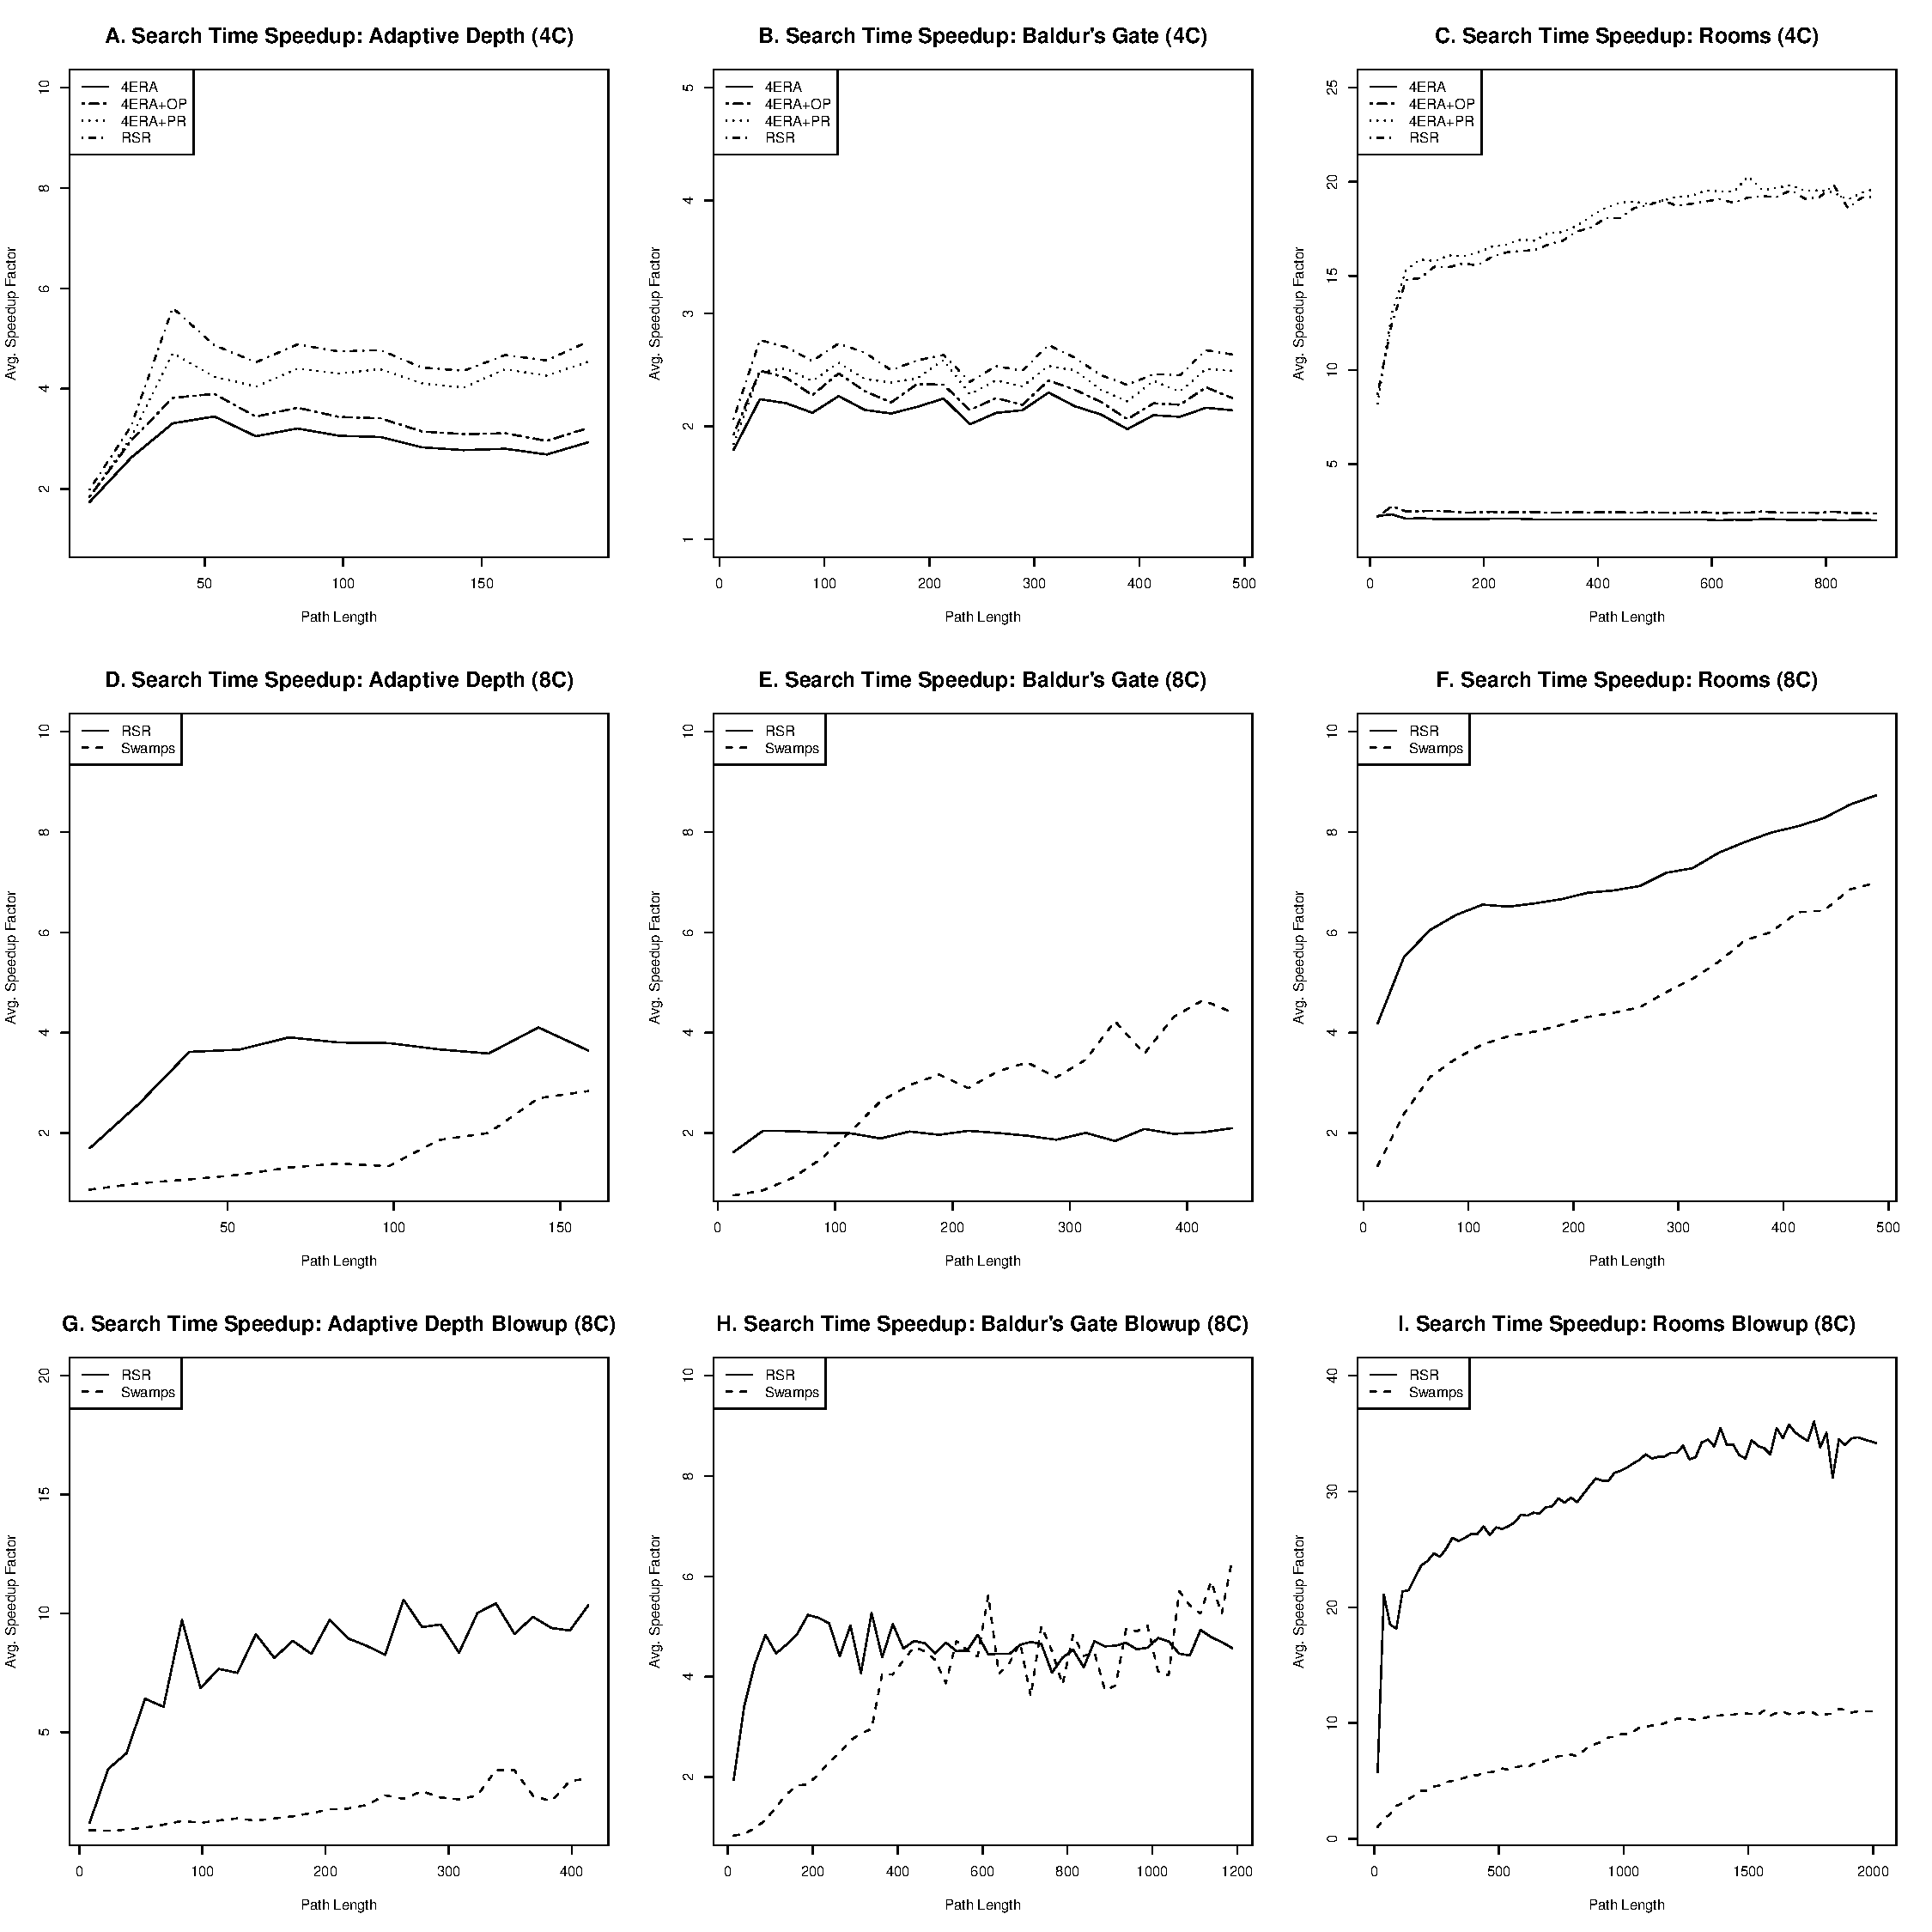
\includegraphics[width=1.95\columnwidth, trim = 10mm 10mm 10mm 0mm]{diagrams/speedup.pdf}
       \end{center}
       \caption{Average A* speedup on each of our three benchmarks. 
		Results are given in terms of nodes expanded and search time.}
\label{fig-speedup}
\end{figure*}

We begin our analysis with Figure \ref{fig-speedup} A-C in which we study the 
effectiveness of our offline perimeter reduction technique (PR) and on-the-fly 
pruning strategy (OP) to speeding up A* search. 
Our baseline comparison is the basic Rectangular Room Symmetry Reduction algorithm 
(RRSR for short) originally described in \cite{harabor10}.
Some clear trends immediately emerge: first, the single biggest improvement in each
case is observed when applying perimeter reduction to the basic RRSR method.
In the case of the Rooms benchmark (Figure \ref{fig-speedup} C) RRSR+PR is over 9
times faster than RRSR alone and up to 19 times faster than A* search on an unmodified
grid map.
Smaller but still significant gains are also observed on the remaining two benchmarks:
on Adaptive Depth (Figure \ref{fig-speedup}A) RRSR+PR is twice as fast as RRSR alone
and performance on Baldur's Gate (Figure \ref{fig-speedup}) is improved by over 10\%.
Combining perimeter reduction with on-the-fly pruning improves these results by a further
10\% in most cases.
The sometimes large performance variation from one benchmark to another is indicative
of how effectively we can decompose the different maps into rectangular shaped regions.
For example, the maps in the Rooms set are highly suited to this approach but those
from Baldur's Gate, which have an unusual 45-degree orientation, are not.
